\chapter{Introduction}
\label{chap_intro}

\ifthenelse{\boolean{wholethesis}}{\relax}{\begin{center}\textit{Generated on \today\ at \currenttime}\end{center}}
\newpage

\section{\label{ch1.sec.history1}From Alchemy to Chemistry}

\lettrine{\initial{F}}{}or nearly 2000 years, scholars believed that everything was made up of combinations of just four elements: air, earth, fire and water. This belief survived until the 17$^\mathrm{th}$ century. One of the first to doubt the original principles was Boyle. In his book \textit{The Skeptical Chymist}, published in 1661, he wrote that matter is composed of elemental particles and that changes in matter are caused by rearrangement of these elemental particles \cite{boyle}. One of the aspects of early chemistry, or alchemy, that Boyle did not challenge was the so-called \textit{phlogiston} theory. Until the 18$^\mathrm{th}$ century, it was generally believed that fire (or \textit{phlogiston}) was part of matter. Metals, for example, were thought to be a combination of earth and fire, because when a metal was burnt the \textit{phlogiston} left the metal and only the residual earth (metal oxide) was left. In 1789 de Lavoisier, writer of the famous book \textit{Trait\'e \'El\'ementaire de Chimie} \cite{lavoisier}, countered this belief by pointing out that this earth, left after burning of the metal, weighed more than the metal itself. With later experiments the existence of oxygen was proven and the increase of weight could now be understood.

Several elements, like carbon and iron have been known from antiquity. In the late 18$^\mathrm{th}$ and early 19$^\mathrm{th}$ centuries more and more elements were discovered, like chromium (Cr), beryllium (Be) and titanium (Ti).  In 1869 Mendeleev ordered the known elements on their mass \cite{mendeleev}. Mendeleev had the audacity to leave open spaces in his table for elements that were not yet discovered. He went even further by predicting some properties of those elements by looking at the properties of elements in the same column. In the subsequent years his predictions were confirmed when the three elements, gallium (Ga), germanium (Ge) and scandium (Sc) were identified, filling their open spaces in the periodic table.

At the dawn of the 20$^\mathrm{th}$ century people, like Thomson and Lewis, were studying the way atoms bind together. Until then atoms were thought to be indivisible, as the Greek word \textit{atomos} implies. Thomson, however, pointed out that the linkages between atoms are caused by the transfer of ``corpuscles'', stating: ``For each valency bond established between two atoms the transference of one corpuscle from the one atom to the other has taken place, the atom receiving the corpuscle acquiring a unit charge of negative electricity, the other by the loss of a corpuscle acquiring a unit charge of positive \cite{thomson}.'' These valency (electrostatic) bonds were schematically represented with arrows (Figure \ref{ch1.fig1}). The carbon atom in methane (CH$_4$) has taken up four electrons, while in tetrachloromethane (CCl$_4$), it has lost four. The arrows indicate the transfer direction of the electrons. 
\begin{figure}[htdp]
\center
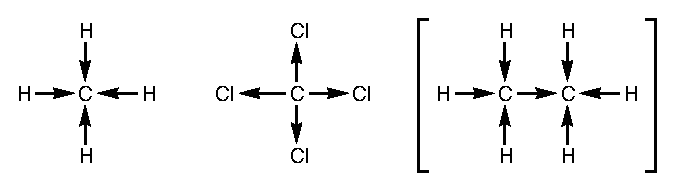
\includegraphics[width=4in]{introduction/figures/figure1.eps}
\caption{Schematic representation of the bonds in methane, tetrachloromethane and ethane \cite{falk}.}
\label{ch1.fig1}
\end{figure}
The situation with the ``equivalent'' carbon atoms in ethane was described by Falk and Nelson: ``In ethane (C$_2$H$_6$), therefore, one of the carbon atoms will have a charge of four units of negative electricity and the other of two units, or comparing the carbon atoms of the two methyl groups, one will be negatively charged and the other positively charged \cite{falk}.'' Thomson, however, already doubted this mechanism and indicated that it was not yet fully understood \cite{thomson}.

In 1916 Lewis introduced a set of postulates still used in chemistry today \cite{lewis}. He refined the classical electrostatic view of Falk and Nelson by writing that the electrostatic forces between particles which are close together do not obey the simple law of inverse squares which holds at greater distances. Lewis also suggested that atoms tend to assume the electronic configuration of a noble gas, through electron transfer or through the sharing of electrons with other atoms, and that the eight outermost electrons in an atom with a noble-gas electronic structure are arranged tetrahedrally in pairs about the atom.
\begin{figure}[htdp]
\center
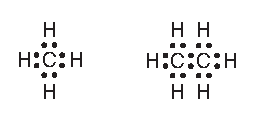
\includegraphics[width=2in]{introduction/figures/figure2.eps}
\caption{The Lewis representation of the bonds in methane and ethane \cite{lewis}.}
\label{ch1.fig2}
\end{figure}
Furthermore, Lewis introduced in this article a new way of representing chemical bonds, which is shown in Figure \ref{ch1.fig2}. These representations show that the carbon atoms in methane, as well as in ethane, acquired a noble-gas configuration, which is known nowadays as the \textit{octet rule} \cite{bruice}.

\section{Quantum Mechanics in Chemistry}

In the 1920s the physicists Heisenberg and Schr\"{o}dinger, amongst others, developed the quantum mechanics. Heisenberg formulated his theory in terms of matrices \cite{heisenberg}, while Schr\"{o}dinger used wave functions \cite{schrodinger1,schrodinger2}. Both formulations are equivalent \cite{schrodinger3}. For the work described in this thesis, only the so-called time independent, non-relativistic Schr\"{o}dinger equation is used:
\begin{equation}
\mathbf{H} \Psi=E \Psi.
\label{ch1.eq.hpsi}
\end{equation}
For each (chemical) system a Hamiltonian ($\mathbf{H}$) can be defined. This Hamiltonian contains terms to obtain the kinetic energy of the nuclei and electrons ($\mathbf{T}_n$ and $\mathbf{T}_e$) and the potential energy of the nuclei and electrons, \textit{i.e.} Coulomb repulsion between nuclei ($\mathbf{V}_{nn}$), Coulomb repulsion between electrons ($\mathbf{V}_{ee}$), and Coulomb attraction between nuclei and electrons ($\mathbf{V}_{en}$):
\begin{equation}
\mathbf{H} = \mathbf{T}_n + \mathbf{T}_e + \mathbf{V}_{nn} + \mathbf{V}_{ee} + \mathbf{V}_{en}.
\label{ch1.eq.htotal}
\end{equation}
By solving equation \ref{ch1.eq.hpsi} all information about the system is accessible. Solving this equation, however, poses a real challenge, since it can only be solved analytically for the simplest cases. For all other systems, like the molecules described in this thesis, approximations are applied.

The first approximation considered is the Born-Oppenheimer approximation \cite{born}. In this approximation, the Hamiltonian is written as a sum of terms for the nuclei and the electrons:
\begin{equation}
\mathbf{H} = \mathbf{H}_n + \mathbf{H}_e = (\mathbf{T}_n + \mathbf{V}_{nn}) + (\mathbf{T}_e + \mathbf{V}_{ee} + \mathbf{V}_{en}).
\label{ch1.eq.hsplit}
\end{equation}
$\Psi$ can then be approximated by a product of a wave function for the nuclei and one for the electrons. Because of the term $\mathbf{V}_{en}$ $\Psi_{e}$ also depends on the coordinates of the nuclei:
\begin{equation}
\Psi \approx \Psi_{n}(\mathrm{X}) \Psi_{e}(\mathrm{q,X}).
\end{equation}
One assumption in the Born-Oppenheimer approximation is that the electronic wave function $\Psi_{e}$ does not change much for small variations in the positions of the nuclei ($\mathrm{X}$) \cite{born}. On the other hand, it is assumed that the motion of the nuclei, which are much heavier than the electrons, does depend on the electron density, rather than on the positions of the individual electrons. With those approximations, the total energy ($E_\mathrm{tot}$) can be written as the sum of a contribution of the nuclei and one of the electrons:
\begin{equation}
E_\mathrm{tot} = \frac{\mathbf{H}_n \Psi_n(\mathrm{X})}{\Psi_n(\mathrm{X})} + \frac{\mathbf{H}_e \Psi_e(\mathrm{q,X})}{\Psi_e(\mathrm{q,X})} = E_{n} + E_{e}.
\end{equation}

Several types of approximations for the wave functions ($\Psi$) have been defined to describe chemical systems. All these wave functions have in common that they are expressed in molecular orbitals ($\psi$), which are linear combinations of atomic orbitals (AOs) $\phi$, or basis functions (LCAO MOs):
\begin{equation}
\psi = c_1 \phi_1 + c_2 \phi_2 + \cdots + c_n \phi_n = \sum_n c_n \phi_n.
\label{ch1.eq.lcaomo}
\end{equation}
The molecular orbitals (MOs) are functions of the coordinates of the electrons (spatial orbitals), or of the coordinates \textit{and} the spins of the electrons (spin orbitals). The spin of an electron can be one of two states. Commonly, these states are referred to as $\alpha$ and $\beta$ spin. The term ``doubly occupied molecular orbital'' indicates that there are two electrons with the same spatial orbital, but with opposite spins.

\subsection{Hartree Products and Slater Determinants}

Multi-electron wave functions are either written as Hartree products \cite{hartree1,hartree2,hartree3} or as Slater determinants \cite{slater}. In a Hartree product the wave function is written as a product:
\begin{equation}
\Psi=\prod_i \psi_i(\mathbf{\tau}_i),
\end{equation}
in which the parameters $\mathbf{\tau}_i$ contain the spatial and spin coordinates of the electrons. This type of wave function is used in the H\"uckel method \cite{huckel1,huckel2,huckel3} (see section \ref{ch1.sec.huckel}). Characteristic for Hartree product wave functions is that they do not fulfil the antisymmetry principle \cite{atkins}. This principle states that the total wave function must change sign when the spatial and spin coordinates of two electrons are interchanged, which is the case when the wave function is written as a determinant. In such a determinant, referred to as Slater determinant in quantum chemistry, the sign of the wave function changes:
\begin{equation}
\begin{split}
\Psi_1 &=
\begin{array}{|cc|}
\psi_1(\mathbf{\tau_1}) & \psi_2(\mathbf{\tau_1}) \\
\psi_1(\mathbf{\tau_2}) & \psi_2(\mathbf{\tau_2}) \\
\end{array}
= \psi_1(\mathbf{\tau_1})\psi_2(\mathbf{\tau_2}) - \psi_1(\mathbf{\tau_2})\psi_2(\mathbf{\tau_1}), \\
\Psi_2 &=
\begin{array}{|cc|}
\psi_1(\mathbf{\tau_2}) & \psi_2(\mathbf{\tau_2}) \\
\psi_1(\mathbf{\tau_1}) & \psi_2(\mathbf{\tau_1}) \\
\end{array}
= \psi_1(\mathbf{\tau_2})\psi_2(\mathbf{\tau_1}) - \psi_1(\mathbf{\tau_1})\psi_2(\mathbf{\tau_2}), \\
\Psi_1 &= - \Psi_2
\end{split}
\label{ch1.eq.slater}
\end{equation}
A nice aspect of writing the wave function as a determinant is that it automatically becomes zero in the case of the occurence of two orbitals with the same spatial \textit{and} spin coordinates. This effect is linked to the Pauli exclusion principle, which practically translates into the rule that no two electrons can occupy the same spin orbital. In that case, the determinant contains two identical columns and hence becomes zero.

Throughout the years, many quantum chemical methods have been developed based on Slater determinants and molecular orbitals (MOs). These methods are described in quantum chemical textbooks \cite{szabo}. Here, the methods used throughout this thesis will be introduced briefly.

\subsection{The Hartree-Fock (HF) Method}
The simplest way to solve the Schr\"{o}dinger equation (equation \ref{ch1.eq.hpsi}) is with the help of a function where the N-electron wave function is approximated by a single Slater determinant (equation \ref{ch1.eq.slater}). This is called the Hartree-Fock method \cite{hartree1,hartree2,hartree3,fock}. For a normalized wave function ($\left< \Psi_\mathrm{HF} | \Psi_\mathrm{HF} \right> = 1$), the energy ($E$) is calculated as an expectation value of the Hamiltonian ($\mathbf{H}$):
\begin{equation}
E=\left< \Psi_\mathrm{HF} | \mathbf{H} | \Psi_\mathrm{HF} \right>,
\label{ch1.eq.hfexp}
\end{equation}
where $\Psi_\mathrm{HF}$ is the single deteminant Hartree-Fock wave function constructed from orthonormal orbitals $\psi_i$.

With the Hamiltonian of equation \ref{ch1.eq.htotal}, the expression for the energy ($E$) becomes:
\begin{equation}
E=\sum_i h_{ii} + \frac{1}{2} \sum_i\sum_j (J_{ij} - K_{ij}) + \mathbf{V}_{nn},
\label{ch1.eq.hfexp_detailed}
\end{equation}
where $h_{ii}$:
\begin{equation}
h_{ii} = \left< \psi_i(\tau_1) | \mathbf{T}_{e}(\tau_1) + \mathbf{V}_{en}(\tau1) | \psi_i(\tau_1)\right>,
\end{equation}
describes the kinetic energy of electron $\tau_1$ and its attraction to the nuclei.

The second term on the right hand side of equation \ref{ch1.eq.hfexp_detailed} contains the so-called Coulomb ($J_{ij}$) and exchange ($K_{ij}$) interactions. These arise from the electron-electron repulsion term $\mathbf{V}_{ee}$ in the Hamilton operator (equation \ref{ch1.eq.htotal}). The exchange interaction is present because Slater determinants are used. This is exemplified with the help of the Slater determinant ($\Psi_1$) of equation \ref{ch1.eq.slater}:
\begin{equation}
\begin{split}
\left< \Psi_1 | \mathbf{V}_{ee} | \Psi_1 \right> = & \left< \psi_i(\mathbf{\tau_1})\psi_j(\mathbf{\tau_2}) | \frac{1}{r_{12}} | \psi_i(\mathbf{\tau_1})\psi_j(\mathbf{\tau_2}) \right> - \\
& \left< \psi_i(\mathbf{\tau_1})\psi_j(\mathbf{\tau_2}) | \frac{1}{r_{12}} | \psi_j(\mathbf{\tau_1})\psi_i(\mathbf{\tau_2}) \right> \\
= & J_{ij} - K_{ij}, \\
\end{split}
\end{equation}
where $\frac{1}{r_{12}}$ is the electron-electron repulsion operator.

Because the Born-Oppenheimer approximation (the motions of nuclei and electrons are split) is applied, the kinetic operator ($\mathbf{T}_{n}$) is absent in equation \ref{ch1.eq.hfexp_detailed}. The nuclei-nuclei repulsion ($\mathbf{V}_{nn}$) adds a constant contribution to the energy ($E$) in equation \ref{ch1.eq.hfexp_detailed} for fixed molecular geometries.

After setting up $\Psi_\mathrm{HF}$ with start-up orbitals, the wave function is optimized in an iterative way. During this process the minimum, or at least a stationary point, is sought for the expectation value $E$ in equation \ref{ch1.eq.hfexp}. For this purpose, the variation principle is applied \cite{varia}. During the optimization the orbitals are modified, but are kept orthonormal. The minimization of the energy with respect to change in the orbitals leads to the following Hartree-Fock equations:
\begin{equation}
\mathbf{F}(i)\psi_j(i)=\epsilon_j \psi_j(i),
\label{ch1.eq.fock1}
\end{equation}
in which $\mathbf{F}(i)$ is the so called one electron Fock operator, which is written as:
\begin{equation}
\mathbf{F}(i)=\mathbf{h}(i) + \sum_j (\mathbf{J_j}(i) - \mathbf{K_j}(i)).
\label{ch1.eq.fock2}
\end{equation}
Since the Fock operator depends on the orbitals it operates on, the Hartree-Fock equations (\ref{ch1.eq.fock1} and \ref{ch1.eq.fock2}) are solved in an iterative manner, referred to as the self consistent Field (SCF) method.

The optimization is performed by modifying the coefficients $c_n$ for the atomic orbitals in equation \ref{ch1.eq.lcaomo}. The Fock operator, expressed in atomic orbitals (AOs), becomes:
\begin{equation}
\mathbf{F}(i)\sum_n c_n \phi_n = \epsilon_j \sum_n c_n \phi_n.
\label{ch1.eq.fockao}
\end{equation}

Equation \ref{ch1.eq.fockao} can be written in matrix form by multiplying from the left with an atomic orbital and integrating:
\begin{equation}
\mathbf{F}\mathbf{C} = \mathbf{S}\mathbf{C}\mathbf{\epsilon},
\label{ch1.eq.fockmatrixs}
\end{equation}
in which $\mathbf{F}$ is the Fock matrix, $\mathbf{S}$ the orbital overlap matrix and $\mathbf{\epsilon}$ the matrix of orbital energies. The $\mathbf{S}$ matrix is present, because the basis functions $\phi_n$ are not orthogonal. However, linear combinations can be chosen in such a way that the basis becomes orthogonal. With such a transformation $\mathbf{S}$ becomes a unity matrix and equation \ref{ch1.eq.fockmatrixs} becomes:
\begin{equation}
\mathbf{F'}\mathbf{C'} = \mathbf{C'}\mathbf{\epsilon}.
\end{equation}

In the Hartree-Fock method the most commonly used type of wave function is a single determinant with doubly occupied orbitals, \textit{i.e.} two electrons per orbital with paired spins. This is referred to as closed-shell and the wave function is called restricted Hartree-Fock (RHF). If not all orbitals are doubly occupied, \textit{i.e.} not all electrons are paired, the wave function is referred to as restricted open-shell Hartree-Fock (ROHF). When different spatial orbitals are used for electrons with $\alpha$ and $\beta$ spin, the method is referred to as unrestricted Hartree-Fock (UHF). An advantage of UHF over ROHF is that it gives a correct description of the dissociation of molecules into atoms or molecular fragments, for example. A disadvantage of UHF, however, is that the wave function is not a proper eigenfunction of the total spin operator $\mathbf{S}^2$.

A property of the single determinant in the Hartree-Fock method is that each electron moves in the average electric field created by the other electrons, \textit{i.e.} there is no electron correlation. For a more accurate expression, the instantaneous interaction between the electrons must be taken into account. Electronic structure methods that take care of electron-electron interaction are called electron correlation methods. The difference between the Hartee-Fock energy ($E_\mathrm{HF}$) and the exact energy is called the \textit{correlation energy}. Three of these methods, the Configuration Interaction Method (CI) \cite{shavitt1,shavitt2}, Multi Configuration Self Consistent Field Method (MCSCF) \cite{daswahl,wahldasbook,mcscf,roos1,roos2} and the Coupled Cluster Method (CC) \cite{cc1,cc2}, will be introduced here.

\subsection{\label{ch1.sec.huckel}The H\"{u}ckel Method}

The H\"uckel method, based on Hartree products, is well suited for the qualitative analysis of $\pi$ electrons in conjugated molecules. Although this method is often used in Chemistry textbooks, it has been actually used as part of the research described in Chapter \chhuckel. Here, the H\"{u}ckel rule, or 4$n$+2 rule for aromatics \cite{bruice}, will be verified with the H\"{u}ckel method.

The $\pi$ orbitals in planar conjugated molecules lie perpendicular to the molecular plane. These orbitals can be expressed as LCAOs of the $2p$ orbitals on the carbon atoms. For ethane this would lead to the molecular orbital $\psi$:
\begin{equation}
\psi=c_A \phi_{A_{2p}} + c_B \phi_{B_{2p}},
\end{equation}
where $\phi_{A_{2p}}$ and $\phi_{B_{2p}}$ are the $2p$ orbitals on carbon atoms A and B, respectively.

\subsection{\label{ch1.sec.ci}The Configuration Interaction (CI) Method}

A Configuration Interaction (CI) wave function is created from a reference function ($\Phi_0$), quite often a Hartree-Fock wave function ($\Phi_0 = \Psi_\mathrm{HF}$), with the help of an excitation operator $\mathbf{T}$:
\begin{equation}
\mathbf{T}=\mathbf{T}_1 + \mathbf{T}_2 + \mathbf{T}_3 + ... + \mathbf{T}_{N_{\mathrm{elec}}},
\label{ch1.eq.ciexcitation}
\end{equation}
in which $\mathbf{T}_1$ is a single excitation operator, $\mathbf{T}_2$ a double excitation operator and $\mathbf{T}_{N_{\mathrm{elec}}}$ the operator that excites \textit{all} $N_{\mathrm{elec}}$ electrons in the molecule. The excitation results in excited Configuration State Functions (CSFs) \cite{shavitt1,shavitt2}. A CSF ($\Phi_k$) is constructed from one or more Slater determinants in such a way that it is an eigenfunction of the N-electrons' spin operators $\mathbf{S}^2$ and $\mathbf{S}_z$. Single and double excited CSF are created by $\mathbf{T}_1$ and $\mathbf{T}_2$, respectively:
\begin{equation}
\begin{split}
\mathbf{T}_1 \Phi_0 & = \sum_i^{occ} \sum_a^{vir} c_i^a \Phi_i^a \\
\mathbf{T}_2 \Phi_0 & = \sum_{i<j}^{occ} \sum_{a<b}^{vir} c_{ij}^{ab} \Phi_{ij}^{ab},
\end{split}
\label{ch1.eq.ciexcited}
\end{equation}
in which $\Phi_i^a$ and $\Phi_{ij}^{ab}$ are singly and doubly excited CSFs, respectively. The total CI wave function ($\Psi_{\mathrm{CI}}$) is constructed from a linear combination of these excited CSFs:
\begin{equation}
\Psi_{\mathrm{CI}} = \sum_{k}^{N_{\mathrm{CSF}}} c_k \Phi_k,
\label{ch1.eq.ci}
\end{equation}
in which $k$ runs over all CSFs. The coefficients $c_k$ are determined by the variational principle \cite{varia}, while the orbitals inside $\Phi_k$ are kept fixed. A wave function containing all possible CSFs in equation \ref{ch1.eq.ci} for a given basis set is called a full CI wave function. Solving the Schr\"{o}dinger equation \ref{ch1.eq.hpsi} gives the ``exact'' energy for that given basis set. In full CI, the number of CSFs is accompanied by a factorial increase with the number of electrons and the size of the basis set \cite{weyl}. Therefore, a full CI wave function is only feasible for very small molecular systems. In practice, the CI expansion is truncated and only a subset of the possible CSFs is included in the wave function. These truncations are labeled with capitals S, D, T, Q to indicate that only singly, doubly, triple, or quadruple excited configurations are included in the expansion. For example, in a CISD wave function only singly and doubly excited CSFs are included in the expansion.

A disadvantage of such a truncation is that the wave function is no longer size consistent, \textit{i.e.} the wave function for a combination of molecules at large distance from each other has a higher energy than the sum of the individual energies. For example, a CISD expanded wave function for a single H$_2$ molecule contains the CSF describing the doubly excited state. Although, for a combination of two H$_2$ molecules at large distance, double excitations do occur within each molecule, the CSF in which \textit{both} H$_2$ molecules are doubly excited at the \textit{same} time does not occur, since this would be a quadruple excitation.

Although CI wave functions have not been used for the calculations described in this thesis, in the Valence Bond Configuration Interaction method, described later in this chapter, the same principle of optimizing the CSF, or structure, coefficients with fixed orbitals is applied.

\subsection{\label{ch1.sec.mcscf}The Multi Configuration Self Consistent Field (MCSCF) Method}
Like in CI, Multi Configuration Self Consistent Field (MCSCF) wave function are expressed in Configuration State Functions (CSFs) \cite{wahldasbook,daswahl}. In contrast with CI, both the orbital \textit{and} the expansion coefficients are optimized in MCSCF.

In MCSCF the Super CI method \cite{superci1,superci2}, in which the wave function is expanded with singly excited structures, is used. For this expanded wave function the CI (or Brillouin) vector $\mathbf{b}$ is determined by solving the generalized eigenvalue problem:
\begin{equation}
[\mathbf{H}-E_b] \cdot \mathbf{b} = 0,
\label{ch1.eq.geig}
\end{equation}
in which $\mathbf{H}$ is the Hamiltonian and in the basis of the ground state and the singly excited states ($\Phi_0$ and the $\Phi_{i}^{a}$s). $E_b$ is the lowest eigenvalue and $\mathbf{b}$ is the corresponding eigenvector. With the elements of $\mathbf{b}$ the orbitals are updated. This procedure is repeated until the Brillouin theorem \cite{brillouin}, which states that for optimal orbitals the singly excited Brillouin states do not interact or mix with the ground (or reference) state, is fulfilled:
\begin{equation}
\left < \Phi_0 | \mathbf{H} - E_0 | \Phi_{i}^{a} \right > = 0.
\label{ch1.eq.brillouin}
\end{equation}

In a special form of MCSCF wave functions the orbitals are divided over two sets. One set contains the orbitals that are doubly occupied in all CSFs (inactive) and the other set contains the variably occupied orbitals (active). In the active space the CSFs are generated by distributing active electrons over the active orbitals in all possible ways. This can be considered as a full CI in the active space. In literature, two designations for this type of method are found. It is referred to as the Fully Optimized Reaction Space (FORS) method \cite{fors1,fors2,fors3} and as Complete Active Space SCF (CASSCF) \cite{roos1,roos2}.

Although MCSCF is not used for calculations described in this thesis, in the Valence Bond Self Consistent field method, described later in this chapter, the same mechanism, \textit{i.e.} Super CI, to optimize the wave function is used (\textit{cf.} Chapter \chorbopt).

\subsection{The Coupled Cluster (CC) Method}
In the coupled cluster method, the wave function is written as an exponential \textit{ansatz} \cite{cc1,cc2}:
\begin{equation}
\Ket{\Psi_{\mathrm{CC}}}  = e^{\mathbf{T}}\Ket{\Phi_{0}},
\end{equation}
in which $e^\mathbf{T}$ contains the excitation operator $\mathbf{T}$ described for CI wave functions (equation \ref{ch1.eq.ciexcitation}). In analogy with CI, a series of excited CSFs is created (equation \ref{ch1.eq.ciexcited}).  The operator $e^{\mathbf{T}}$ can be expanded as a Taylor series:
\begin{equation}
e^{\mathbf{T}} = 1 + \mathbf{T} + \frac{1}{2!}\mathbf{T}^2 + \frac{1}{3!}\mathbf{T}^3 + ... = \sum_{k=0}^{\infty} \frac{\mathbf{T}^k}{k!}
\label{ch1.eq.taylor}
\end{equation}
From equations \ref{ch1.eq.ciexcitation} and \ref{ch1.eq.taylor} the exponential operator (up till $\mathbf{T}_4$) may be written as:
\begin{equation}
\begin{split}
e^{\mathbf{T}} = & 1 + \mathbf{T}_1 + (\mathbf{T}_2 + \frac{1}{2}\mathbf{T}_1^2) + (\mathbf{T}_3 + \mathbf{T}_2\mathbf{T}_1 + \frac{1}{6}\mathbf{T}_1^3) + \\
& (\mathbf{T}_4 + \mathbf{T}_3\mathbf{T}_1 + \frac{1}{2}\mathbf{T}_2^2 + \frac{1}{2}\mathbf{T}_2\mathbf{T}_1^2 + \frac{1}{24} \mathbf{T}_1^4) + ...
\end{split}
\end{equation}
The first term on the right hand side generates the reference $\Phi_0$ and the second term ($\mathbf{T}_1$) all singly excited states. The third term (the first between brackets) generates all doubly excited states, which may be considered as connected ($\mathbf{T}_2$) or disconnected ($\mathbf{T}_1^2$). The fourth term  generates all triply excited states and the last term the quadruples. Physically, a connected type such as $\mathbf{T}_4$ corresponds to four electrons interacting simultaneous, while a disconnected term such as $\mathbf{T}_2^2$ corresponds to two non-interacting pairs of interacting electrons. By comparison with the CI wave function, it is seen that the CC wave function at each excitation level contains additional terms arising from products of excitations \cite{jensen}. The coupled cluster method is size consistent, if the reference wave function ($\Phi_0$) is.

Like in CI, the excitation level is truncated in practice. Commonly used levels of coupled cluster are single, double and triple, CCS, CCSD and CCSDT, respectively. CCSDT gives good correlation energies and is accurate. However, the inclusion of the triple excitations makes this method very compute intensive. The designation CCSD(T), with the T between brackets, indicates that the triple excitations are approximated by perturbation theory rather than computed, making it less compute intensive.

\subsection{Density Functional Theory (DFT)}
The central goal of all methods described so far is to solve the time independent Schr\"{o}dinger equation (equation \ref{ch1.eq.hpsi}). This is also the goal of the Density Functional Theory (DFT) \cite{jensen, hohenberg, kohnsham}, but the approach is different. The most compute intensive operator in the Hamiltonian is the electron-electron repulsion term ($\mathbf{V}_{ee}$). The idea of DFT is to solve the Schr\"{o}dinger equation by means of a density function instead of the electon-electron repulsion operator.

The density function is defined as:
\begin{equation}
\rho(r_1)=n \int ds_1dr_2ds_2 ... dr_nds_n | \Psi(r_1,s_1,r_2,s_2, ... r_n,s_n)|^2,
\end{equation}
where $r_1$ and $s_1$ stand for the spatial and spin coordinates of electron one, respectively. The first Hohenberg-Kohn theorem, central to DFT, states that a bijection relation of the external potential and the ground state density function exits. This means that the ground state density function is uniquely set by the external potential and
that the external potential is unambiguously determined by the ground state density function:
\begin{equation}
\rho^0(\mathbf{r}) \Leftrightarrow v^{ext}(\mathbf{r}).
\end{equation}

Like in wave function methods, described before, Kohn and Sham introduced orbitals into DFT. These orbitals are describing an external N-electron system that has the same density function as the real N-electron system, without the electron-electron repulsion. The corresponding density function is:
\begin{equation}
\rho(\mathbf{r}) = \sum_i | \psi_i(\mathbf{r})|^2.
\label{ch1.eq.kohnsham1}
\end{equation}
The one electron Hamilton operator per orbital $i$ then becomes:
\begin{equation}
\left( -\frac{1}{2} \sum_i \nabla^2_i + v_s (\mathbf{r}) \right) \psi_i(\mathbf{r}) = \epsilon_i\psi_i(\mathbf{r}),
\label{ch1.eq.kohnsham2}
\end{equation}
where the first term is the kinetic energy operator and $v_s(\mathbf{r})$ the external effective potential. In practice, finding an appropriate $v_s(\mathbf{r})$ is a challenge. The equations \ref{ch1.eq.kohnsham1} and \ref{ch1.eq.kohnsham2} are solved iteratively with the variational principle \cite{varia}.

Throughout this thesis, DFT calculations are mainly used to find optimal equilibrium geometries. On top of these geometries, other types of (Valence Bond) wave functions are constructed for analyzing properties of the molecules at hand.

\section{The Valence Bond Method}

In the previous sections, several quantum chemistry methods were introduced based on the orthonormal molecular orbital method. These methods are used throughout this thesis to support yet another quantum chemical method. To introduce it, the historical chronology of section \ref{ch1.sec.history1} is continued.

Shortly after the birth of quantum mechanics the idea that a chemical bond is made up of a pair of shared electrons between two atoms, as proposed by Lewis, was substantiated. In 1927, Heitler and London wrote that a system containing two neutrally charged hydrogen atoms at close distance is more stable (has a lower energy $E$ (equation \ref{ch1.eq.hpsi})) than a system built from two atoms at infinite distance \cite{heitler}. Later, this mathematical representation of the chemical bond by Heitler and London became known as the Valence Bond (VB) theory. 

In the following decades Linus Pauling incorporated both the postulates of Lewis and VB theory into his view on the nature of the chemical bond \cite{pauling1,pauling2,pauling3,pauling4,pauling5,pauling6,pauling7,paulingbook}, which earned him the Nobel prize in 1954. In the 1950s a lot of dispute arose about the VB theory, because of the numerical sluggishness, mainly caused by the use of non-orthogonal orbitals, and apparent failures like the wrong prediction of the ground state of the oxygen molecule (O$_2$ singlet instead of triplet) \cite{carsten}, the prediction of \textit{aromatic} character in cyclobutadiene (C$_4$H$_4$), C$_5$H$_{5}^{+}$, C$_3$H$_{3}^{-}$ (all with $4$ $\pi$ electrons; \textit{anti-aromatic} according to H\"{u}ckel's rule $4n$, $n=1$ \cite{march}) and in C$_7$H$_{7}^{-}$ (8 $\pi$ electrons; $4n$, $n=2$) and the prediction of \textit{anti-aromatic} character in C$_5$H$_{5}^{-}$, C$_7$H$_{7}^{+}$ (6 $\pi$ electrons; \textit{aromatic} according to H\"{u}ckel's rule $4n+2$, $n=1$) and C$_3$H$_{3}^{+}$ ($4n+2$, $n=0$). Shaik and Hiberty showed that these iconic VB ``failures'' are caused by the use of oversimplified VB models \cite{antibrush}. The correct prediction of the ground state of O$_2$ has been the subject of much discussion since the 1930s \cite{o2_1,o2_2,o2_3,o2_4,o2_5,o2_6,o2_7,o2_8,o2_9,carsten}. Calculations performed by Byrman \textit{et al.}, for example, indicate that the correct triplet ground state is found when the bond between the atoms is considered to be a combination of one $\sigma$ bond and two three electron $\pi$ bonds \cite{carsten}. The singlet ground state will be found when the bond is considered to be a combination of one $\sigma$ and one $\pi$ bond.

A short time after the introduction of the Valence Bond theory, Hund and Mulliken, amongst others, developed the Molecular Orbital theory \cite{hund,mulliken}, on which the Hartree-Fock (HF) method and the other methods described in the previous section are based. Because of the relative easiness to implement the HF model (lower mathematical complexity due to a single determinant wave function with orthogonal molecular orbitals/vectors) and the lower computational efforts compared to VB, the MO method became very popular in the computer era.

Although the interest in VB theory diminished, it was not completely abandoned \cite{vboverv1,vboverv2,vboverv3}. In the following sections it will be made clear that Valence Bond theory must be applied to areas, where it is suited for: the understanding of molecules and chemical behavior in terms of Lewis, or resonance structures, \textit{e.g.} the description of (complex) bond situations.

\subsection{Classical Valence Bond}

The first application of the VB method was for the description of the hydrogen molecule by Heitler and London \cite{heitler}. They used the wave function:
\begin{equation}
\Psi = |1s_{A}\overline{1s_{B}}| - |\overline{1s_{A}}1s_{B}|,
\label{ch1.eq.hl}
\end{equation}
in which $1s_{A}$ and $1s_{B}$ are atomic orbitals centered on the two hydrogen atoms, referred to as $A$ and $B$.
\begin{figure}[htdp]
\center
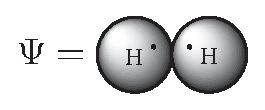
\includegraphics[scale=1]{introduction/figures/heitler.eps}
\caption{Graphical representation of the VB wave function for $\mathrm{H_2}$. The electrons in the two 1$s$ orbitals form a singlet pair.}
\label{ch1.fig.heitler}
\end{figure}
The two determinants together form the VB structure in which the two electrons are spin-coupled into a pair. A graphical representation is shown in Figure \ref{ch1.fig.heitler}. This VB structure represents the Lewis structure $\mathrm{[H^\bullet H^\bullet]}$ for H$_2$, as stressed by Pauling \cite{hllewis}. 

In the years following the introduction of VB, extra versatility was acquired by the expansion of the Valence Bond wave function into multiple structures. For H$_2$ this expansion corresponds to the addition of two ionic structures:
\begin{equation}
\Psi = c_1 (|1s_{A}\overline{1s_{B}}| - |\overline{1s_{A}}1s_{B}|) + c_2 |1s_{A}\overline{1s_{A}}| + c_3 |1s_{B}\overline{1s_{B}}|,
\label{ch1.eq.hlplus}
\end{equation}
in which the third determinant corresponds to the Lewis structure $\mathrm{[H^{-} H^{+}]}$ and the fourth determinant to $\mathrm{[H^{+} H^{-}]}$. A graphical representation is shown in Figure \ref{ch1.fig.heitlerplus}.
\begin{figure}[htdp]
\center
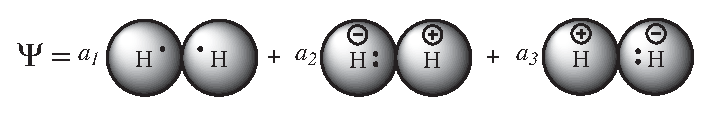
\includegraphics[scale=1]{introduction/figures/heitlerplus.eps}
\caption{Graphical representation of the VB wave function for $\mathrm{H_2}$ with a covalent and two ionic structures. The two bonding electrons are equally shared in the first structure. Both electrons are on the left hydrogen in the second structure and on the right hydrogen in the third structure.}
\label{ch1.fig.heitlerplus}   
\end{figure}
The coefficients $c_1$, $c_2$ and $c_3$ are variationally determined \cite{varia}. The total energy ($E_\mathrm{tot}$) calculated with the $\Psi$ in equation \ref{ch1.eq.hlplus} proved to be lower than the energy calculated with the $\Psi$ in equation \ref{ch1.eq.hl}. In general, for covalent bonds, like H--H, the coefficients $c_2$ and $c_3$ will be non-zero, indicating that they are not merely covalent in nature, but that they also contain some ionic character. This ionic character is caused by the freedom for the electrons to move towards the other atom. For the bond description in VB it is vital that the orbitals are non-orthogonal. The overlap of two singly occupied orbitals on separate atoms or fragments, like the hydrogen atoms mentioned above, can be used as measure for the bond strength. When the two atoms are brought together from infinity to equilibrium distance, the total energy ($E_\mathrm{tot}$) of the molecule decreases as the orbital overlap increases. This suggests that for bonds with ``high overlap'' more energy is required to break it than for bonds with ``low overlap''. This has to be used with caution, though, because at distances below the equilibrium distance, the nuclear repulsion increases so rapidly that this effect will overshadow the still increasing orbital overlap.

The importance (or contribution) of each VB structure to the wave function can be obtained by using the formula of Chirgwin and Coulson \cite{chirgwin}. With their formula weights ($W_j$) can be assigned to the VB structures:
\begin{equation}
W_{j}=\sum_{i} c_{i}c_{j}S_{ij},
\label{ch1.eq.weight}
\end{equation}
in which $S_{ij}$ is the overlap between structure $i$ and $j$ and $c_i$ and $c_j$ are the structure coefficients. For H$_2$ this results in a weight of 0.86 for the covalent $\mathrm{[H^\bullet H^\bullet]}$ structure and 0.07 for both ionic, $\mathrm{[H^{+} H^{-}]}$ and $\mathrm{[H^{-} H^{+}]}$, structures. 

Instead of the homonuclear system H$_2$, one could investigate heteronuclear systems in the same terminology. With the three structures $\mathrm{[A^\bullet B^\bullet]}$, $\mathrm{[A^{+} B^{-}]}$ and $\mathrm{[A^{-} B^{+}]}$ one can study bond polarity and dissociation behavior. This is an application area for VB, as will be exemplified by the following heteronuclear ``molecule''.

The prototype of an electrostatic, or ionic, bond is the one between sodium and chlorine in \mbox{Na--Cl}. As for H--H, a wave function consisting of three structures can be formulated:
\begin{equation}
\Psi = c_1 \cdot \mathrm{[Na^\bullet Cl^\bullet]} + c_2 \cdot \mathrm{[Na^{+} Cl^{-}]} + c_3 \cdot \mathrm{[Na^{-} Cl^{+}]},
\label{ch1.eq.nacl}
\end{equation}
in which determinants comparable to those in equations \ref{ch1.eq.hl} and \ref{ch1.eq.hlplus} have been replaced by Lewis structures for clarity. Throughout this thesis the terms Lewis structure and VB structure are intermixed on several occasions. The reader should be aware that VB structures are not necessarily independent as the pictorial Lewis structures suggest. This is indicated by the possible overlap of the structures in a VB wave function ($S_{ij}$ in equation \ref{ch1.eq.weight}). In practice, VB structures frequently have a non-zero overlap, although they describe different Lewis structures. So, also for the analysis of a chemical bond with a wave function containing only one ionic structure some covalent character is automatically included. Because, when a covalent structure would be added, the overlap of the two structures would not necessarily be zero.

In the $\mathrm{[Na^{+} Cl^{-}]}$ structure, both sodium and chlorine fulfill Lewis' octet rule. The weights of these structures (equation \ref{ch1.eq.weight}) indicate the bond character or polarity of the bond. At equilibrium distance the weight for the $\mathrm{[Na^{+} Cl^{-}]}$ structure is the highest, being 0.75. The covalent $\mathrm{[Na^\bullet Cl^\bullet]}$ structure has a weight of 0.25, while the other ionic structure $\mathrm{[Na^{-} Cl^{+}]}$ does not contribute to the wave function at all. This VB result corresponds to an electrostatic bond. At infinite distance however, the weight for \mbox{$\mathrm{[Na^\bullet Cl^\bullet]}$} equals one, while the weights for the other two structures will be equal to zero. This corresponds to the description of separate neutral atoms.

Another application area is the study of stability in terms of resonance and aromaticity. Resonance is a long known chemical concept, which accounts for stability in molecules, or molecular fragments \cite{whelandbook}. An everyday example is acetic acid (``vinegar'', p$K_\mathrm{a}$~=~4.76 \cite{bruice}). The reason for the acidity of acetic acid is ascribed to the stability of the acetate anion (Figure \ref{ch1.fig.acetic}).
\begin{figure}[htdp]
\center
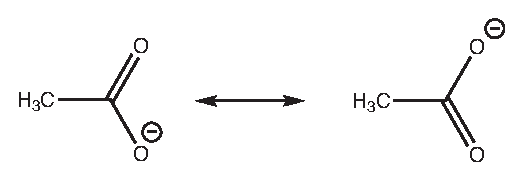
\includegraphics{introduction/figures/acetic.eps}
\caption{The two Lewis resonance structures of the acetate anion, \textit{viz.} the conjugated base of acetic acid.}
\label{ch1.fig.acetic}
\end{figure}
When a proton is abstracted from acetic acid in aqueous environment, the negative charge has to be divided over the acetate anion. After inspection of the Lewis structures in Figure \ref{ch1.fig.acetic} it becomes evident that the negative charge can be positioned on either of the two oxygen atoms, leading to two resonance structures. In contrast, alkanols are known to be very weak acids. For alkanols there is only one resonance structure, in which the negative charge is solely concentrated on the oxygen atom (Figure \ref{ch1.fig.alcohol}).
\begin{figure}[htdp]
\center
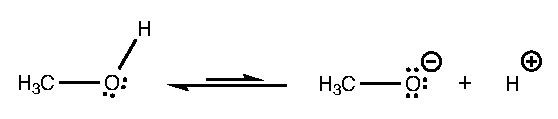
\includegraphics{introduction/figures/alcohol.eps}
\caption{The deprotonation reaction of methanol (an alkanol; p$K_\mathrm{a}$=15.5 \cite{bruice}). On the right side is the only possible resonance structure.}
\label{ch1.fig.alcohol}
\end{figure}
This resonance effect can be explicitly quantified with the Valence Bond method by calculating the Pauling resonance energy \cite{paulingbook}, which is defined as the difference between the energy of the most stable structure and the energy of the total wave function. 

Resonance energy is often used in discussions on aromaticity. In the 19$^\mathrm{th}$ century Michael Faraday discovered benzene, to which he referred to as bicarburet of hydrogen \cite{faraday,bicarburet}. The molecular weight of 78 suggested that the gross formula was (CH)$_6$. A remarkable property of (CH)$_6$ is that, in contrast to other unsaturated carbon based compounds (such as alkenes), benzene does not give addition products, but only substitution products \cite{bruice}. After several scientists suggested different structural formulae, the planar hexagonal structure of August Kekul\'e \cite{kekule} was generally accepted as the real structure (Figure \ref{ch1.fig.benzene}). 
\begin{figure}[htdp]
\center
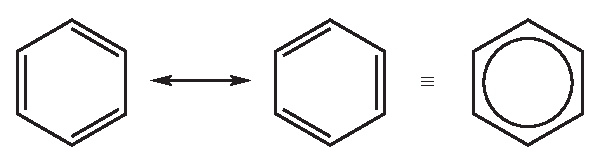
\includegraphics{introduction/figures/benzene.eps}
\caption{The two Kekul\'e resonance structures of benzene (left) and the delocalized electron representation (right).}
\label{ch1.fig.benzene}
\end{figure}
The stability of benzene was ascribed to the delocalization of the 6 $\pi$ electrons, expressed in the resonance between the two Kekul\'e structures.

The Valence Bond wave functions described so far (equations \ref{ch1.eq.hl},\ref{ch1.eq.hlplus} and \ref{ch1.eq.nacl}) are of the classical type. Modern Valence Bond wave functions do not necessarily describe the bonding between separate atoms, but can also describe the bonding between molecular fragments. On these molecular fragments the orbitals can be expressed as linear combinations of atomic orbitals (AOs) available for that fragment. It is more appropriate to denote these functions as molecular orbitals (MOs), since they can spread over several atoms. 

In modern type Valence Bond wave functions atomic and molecular orbital models can also be mixed. For example, a commonly used VB wave function for benzene consists of complete MO description containing the core (the inner shell AOs, \textit{i.e.} the $1s$ orbitals on carbon) and the $\sigma$ system (the valence shell AOs in the plane of the molecule (X-Y), \textit{i.e.} the $2s$, $2p_x$, $2p_y$ orbitals on carbon and the $1s$ orbitals on hydrogen), while the $\pi$ system is described by atomic $2p_z$ orbitals. The total wave function $\Psi_{tot}$ then becomes an antisymmetrized product of an MO wave function for the core-$\sigma$ system and a VB wave function for the $\pi$ system:
\begin{equation}
\Psi_{tot} = \mathcal{A}(\Psi_{\mathrm{core}-\sigma} \times \Psi_{\pi}),
\label{ch1.eq.prodbenzene}
\end{equation}
in which $\mathcal{A}$ is an anti-symmetrizer. The separation of the core-$\sigma$ and $\pi$ systems does not mean that the two are independent, because the electrons in the core-$\pi$ system will ``feel'' the Coulomb repulsion from the electrons in the $\sigma$ system ($\sigma$-$\pi$ interaction).

In the remainder of this section the three types of Valence Bond wave functions supported by TURTLE \cite{turtle}, the VB module in GAMESS-UK \cite{gamess}, are discussed. These are 1) the Generalized Valence Bond (GVB), 2) the Valence Bond Configuration Interaction (VBCI) and 3) the Valence Bond Self Consistent Field (VBSCF \cite{vbscf1,vbscf2}) models. The latter two types of models are compared to their orthogonal analogues and exemplified with a calculation on benzene. For VBSCF both the delocalized as well as the localized orbital models and the Breathing Orbital Valence Bond (BOVB \cite{bovb1,bovb2,bovb3}) method extension are described. Finally, the SCVB ethod \cite{scvb1,scvb2,scvb3} is briefly introduced in this section.

\subsection{Generalized Valence Bond (GVB)}

In the Generalized Valence Bond (GVB) method \cite{jensen,gvb1,gvb2,gvb3,gvb4}, two non-orthogonal orbitals are used to describe a pair of electrons in a bond. Each such pair is coupled to a singlet. Besides these spin-paired singly occupied orbitals, other doubly occupied orbitals may be used. The doubly occupied orbitals and the spin-coupled pairs are chosen orthogonal to each other to reduce the computational effort required. This is called the Strong Orthogonality (SO) condition. The total spin for such a system thus is also singlet. This is known as Perfect Pairing (PP), and is one of the many possible spin coupling schemes, and such two-electron two-orbital pairs are called geminal pairs. A geminal is a wave function for two electrons. 

This type of Valence Bond wave function is used in Chapter \chdissociation\ to generate the geometries on the dissociation curves. For dissociation purposes, a Hartree-Fock wave function does not suffice, since it is not capable of describing a molecule consisting of two radical fragments at large distance from each other.

\subsection{Valence Bond Configuration Interaction (VBCI)}

As the name suggests, there is a strong analogy between the Valence Bond Configuration Interaction Method (VBCI) and Configuration Interaction (section \ref{ch1.sec.ci}). In both cases the orbitals are not optimized in the expansion, but rather only the structure (VB) or CSF (CI) coefficients. A difference between the two is that in the VB case, there is no orthogonality restriction between the orbitals, while in CI the orbitals are orthogonal.

A typical VBCI wave function used in TURTLE consists of several VB structures representing distinctive Lewis structures like the wave function in equation \ref{ch1.eq.hlplus}. Although the bond in H$_2$ is typically covalent in nature, the two ionic structures are included. The effect of the inclusion of the two ionic structures is that the electron on one hydrogen atom gets more freedom to move towards the other hydrogen atom. Even for the covalent bond in H$_2$ this results in a total weight for the ionic structures of 14\% and a lower total energy (\textit{vide supra}) indicating that including these structures improves the wave function.

In the last few years Wu \textit{et al.} have published some articles on VBCI \cite{vbci_wu1,vbci_wu2}. A difference between the implementation in TURTLE and Xiamen \cite{xiamen} is that in TURTLE \textit{any} selection of structures in the expansion and of the orbitals is allowed, while in Xiamen the possibilities for selection are predefined. To start with the latter difference, Wu \textit{et al.} take the orbitals from a preceding VBSCF (\textit{vide infra}) calculation as starting point, while in TURTLE any orbital set may be chosen. For the expansion of the structures any imaginable structure may be included in TURTLE, while the expansion in Xiamen are created by external excitations from a reference structure. In a structure with external excitations one or more occupied orbitals are replaced by empty, or virtual, orbitals. Internal excitations are excitations to orbitals which are vacant in some structures. An example of such an excitation is from $\mathrm{[H^\bullet H^\bullet]}$ to $\mathrm{[H^{+} H^{-}]}$, \textit{i.e.} from $1s_A$ to $1s_B$ once for $\alpha$ and once for $\beta$ spin. Wu defines three levels of expansion: in VBCI(S,S) only singly excited structures are involved. In VBCI(D,S) the active shell, \textit{e.g.} the orbitals in $\Psi_{\pi}$ in benzene (equation \ref{ch1.eq.prodbenzene}), is treated by single and double excitations, whereas the inactive shell, \textit{e.g.} $\Psi_{\mathrm{core}-\sigma}$, is expanded with single excitations only. Also included in this level are double excitations which consist of a single excitation from each shell. In VBCI(D,D) single and double excitations are involved for both active and inactive electrons.

An example of a VBCI wave function is the wave function for benzene, C$_6$H$_6$, in which the $\pi$ system ($\Psi_{\pi}$) is constructed of atomic $2p_z$ orbitals and the core-$\sigma$ system of 18 doubly occupied orbitals. With 6 $\pi$ electrons, 6 $2p_z$ orbitals and all possible bonding arrangements a wave function consisting of 175 structures can be defined (Figure \ref{ch1.fig.structures2}). 
\begin{figure}[htbp]
\center
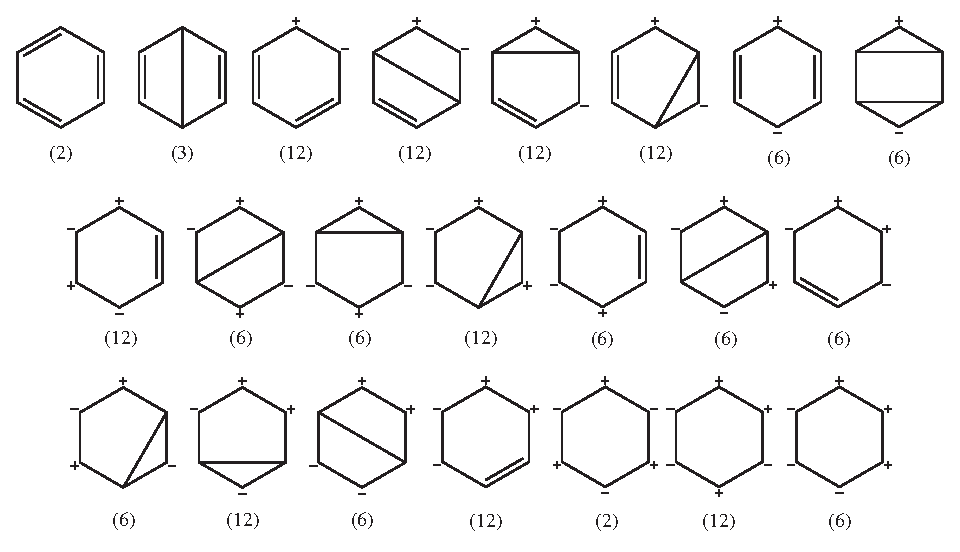
\includegraphics[scale=0.9]{introduction/figures/allstructures.eps}
\caption{The covalent and ionic structures for benzene (with the number of occurrences in brackets): the covalent structures are represented by two Kekul\'e and three Dewar structures. In addition there are 170 ionic structures, giving a total of 175 structures \cite{chembrit}.}
\label{ch1.fig.structures2}
\end{figure}
When all 6 $\pi$ electrons are equally divided over the 6 $2p_z$ orbitals, 5 distinctive bonding arrangements (or spin-couplings) can be made. Two of these are the Kekul\'e structures (Figure \ref{ch1.fig.benzene}). In Figure \ref{ch1.fig.structures2} only one Kekul\'e structure is shown. Beneath it, the number (2) indicates that there are two similar structures in the wave function. The other three bonding arrangements are the Dewar structures (Figure \ref{ch1.fig.structures2}, top row, second from the left), which have a bond across the ring. The other structures in Figure \ref{ch1.fig.structures2} have at least one doubly occupied and one vacant $2p_z$ orbital, resulting in negative and positive charges on the affected carbon atoms, respectively. Several people have used this wave function \cite{vbci175_1,vbci175_2}. Without performing orbital optimizations in the VB model, the total energy ($E_\mathrm{tot}$) for this wave function was found to be lower than that of a single determinant Hartree-Fock wave function with optimized molecular orbitals (MOs). This means that this VBCI wave function has an expectation value for the total energy closer to the best obtainable energy value, \textit{i.e.} the full CI (Configuration Interaction) energy. 

However, the interpretation of the wave function in terms of structure contributions and structure energies proved not  to be trivial. Together with the expected high weights for the Kekul\'{e} structures ($W$=0.222=2x0.111 \cite{vbci175_2}) and, slightly less, the Dewar structures ($W$=0.110=3x0.037), also the orthoionic terms (Figure \ref{ch1.fig.structures2}, top row, third from the left) had a high weight ($W$=0.251=12x0.021). So, looking at single structure contributions, the Kekul\'e structures were most important with a weight of $W$=0.111 per structure. However, looking at the total contribution of a structure type, the orthoionic type, with 12 occurences, were the most important.

To make the wave function more interpretable a VBCI wave function with only the Kekul\'{e} and Dewar structures was used. The results proved to be in line with earlier semi-empirical work on benzene by Craig \cite{craig}. Unfortunately, the energy for this wave function proved to be higher than that of a Hartree-Fock wave function, further from the Full CI energy. Obviously, by excluding the ionic terms, important information for the description of the $\pi$ system was discarded.

In general, an advantage of VBCI is that it can deliver quantitative good results. However, such calculations often require a large number of structures. When many structures have a significant contribution to the wave function the clear Lewis picture may become obscured. Including too few structures on the other hand may lead to a nice interpretable qualitative picture with low quantitative accuracy. 

\subsection{\label{ch1.sec.vbscf}Valence Bond Self Consistent Field (VBSCF)}

In contrast with VBCI, both the orbital \textit{and} the expansion coefficients are optimized. This is analogous to the Multi Configuration Self Consistent Field method (MCSCF) (section \ref{ch1.sec.mcscf}). A VBSCF wave function is  expressed in structures, which are the non-orthogonal equivalent of the Configuration State Functions (CSFs) in MCSCF.  Two major differences are that both bonding \textit{and} anti-bonding orbitals occur in CSFs and that the molecular orbitals (MOs) are chosen orthogonal in MCSCF.

Like in MCSCF, in VBSCF the Super CI method \cite{superci1,superci2}, in which the wave function is expanded with singly excited structures, is used. For VBSCF, however, the overlap matrix between the structures ($\mathbf{S}$) enter the equation (compare with MCSCF in equation \ref{ch1.eq.geig}). Likewise, the  Brillouin vector is determined by solving the generalized eigenvalue problem:
\begin{equation}
[\mathbf{H}-E_b\mathbf{S}] \cdot \mathbf{b} = 0,
\label{ch1.eq.geigvb}
\end{equation}
in which $\mathbf{H}$ and $\mathbf{S}$ are the Hamiltonian and metric in the basis of the ground state and the singly excited states ($\Psi_0$ and the $\Psi_{ia}$'s). $E_b$ is the lowest eigenvalue and $\mathbf{b}$ is the corresponding eigenvector. With the elements of $\mathbf{b}$ the orbitals are updated (for details  \textit{cf.} Chapter \chorbopt), like in equation \ref{ch1.eq.brillouin}.

Cooper, Gerratt and Raimondi investigated benzene with a VB wave function in which they optimized the orbitals \cite{nature}. In their wave function the core-$\sigma$ part was frozen, or kept constant, while the singly occupied $\pi$ orbitals were expressed as linear combinations of the 6 atomic $2p_z$ orbitals. This meant that the $\pi$ orbitals could spread out over the whole $\pi$ system during the optimization process. As Cooper showed, the advantage of the use of a VB wave function with optimized orbitals is that it gives good quantitative results with only a few VB structures: addition of the 170 ionic structures (Figure \ref{ch1.fig.structures2}) to this wave function only resulted in a small energy lowering. Although the orbitals were allowed to spread over the whole $\pi$ system, the orbitals remained centered on the carbon atoms with tails on the neighboring carbons (Figure \ref{ch1.fig6}, top). 
\begin{figure}[htbp]
\center
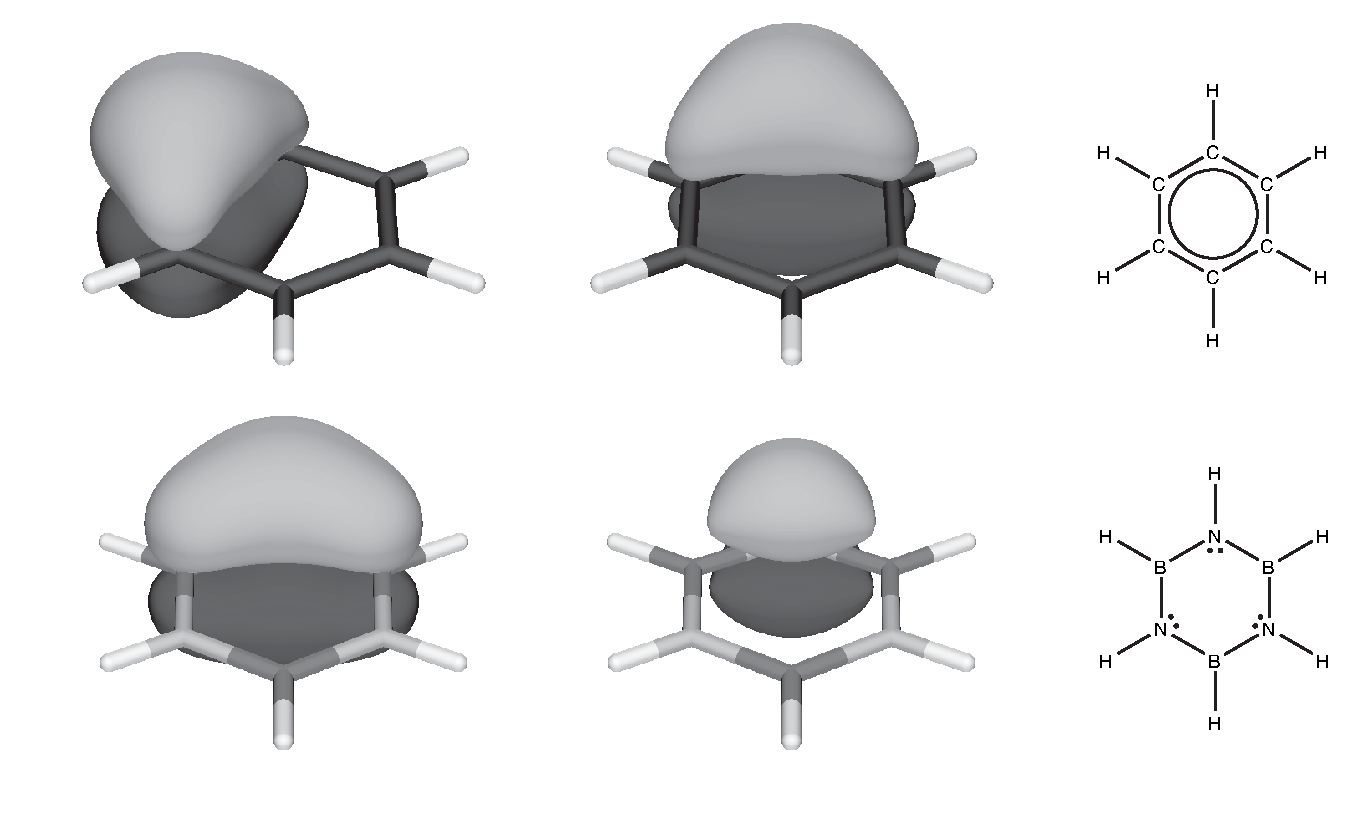
\includegraphics[scale=0.5]{introduction/figures/figure6.eps}
\caption{A set of singly occupied $p$ orbitals on benzene (top) and on borazine (bottom). In these orbital plots the boron atoms are dark colored and the nitrogen atoms light.}
\label{ch1.fig6}
\end{figure}
The orbitals in these plots, made with Molden \cite{molden}, are taken from a VBSCF calculation (\textit{cf.} Chapter \chinorganic). They are, however, equivalent with the contour plots of the SCVB orbitals as published by Cooper \textit{et al.} in Nature \cite{nature}.

A molecule which is iso-electronic with benzene and which also has a planar hexagonal structure is borazine (see the structural formulae on the right hand side in Figure \ref{ch1.fig6}: top - benzene; bottom - borazine). Although both molecules have 6 $\pi$ electrons, their electron contribution is rather different. In benzene, each carbon atom contributes one $p$ electron, while in borazine only the nitrogen atoms contribute two $p$ electrons each. VBSCF calculations with initial atomic $p$ orbitals on each atom of both hexagonal molecules show that the $p$ orbitals remain more or less centered on the initial carbon atom in the case of benzene,  while in the case of borazine an atomic $p$ orbital, which originated on a boron atom, migrated to a neighboring nitrogen atom (with tails remaining on the boron atoms), forming a (localized) lone-pair description with the $p$ orbital already present there (Figure \ref{ch1.fig6}, bottom).

In some cases, due to the increased flexibility of the wave function, the orbitals might no longer be centered on an atom or a bond, but spread out over the whole molecule. In those situations, the interpretability is obscured. In a normal VBSCF calculation all MOs are expressed in all AOs. As a consequence, MOs can completely migrate from one atom to another atom, or fragment during orbital optimization and become \textit{delocalized}. In TURTLE it is possible to specify the AOs available for each MO. During the optimization process these MOs are not allowed to mix in AOs not initially specified. This keeps the MOs \textit{localized}. 

An example of a molecule which is constructed from two fragments with \textit{localized} orbitals is CpSiH (Figure \ref{ch1.fig7}). To investigate the type of bonding between the main group metal Si and the cyclopentadienyl (Cp) ring, two covalent ([Cp$^\bullet$SiH$^\bullet$]) structures and one ionic ([Cp$^{-}$SiH$^{+}$]) structure were defined. In these structures the orbitals on the Cp ring were completely separated from the orbitals on the SiH group.
\begin{figure}[htbp]
\center
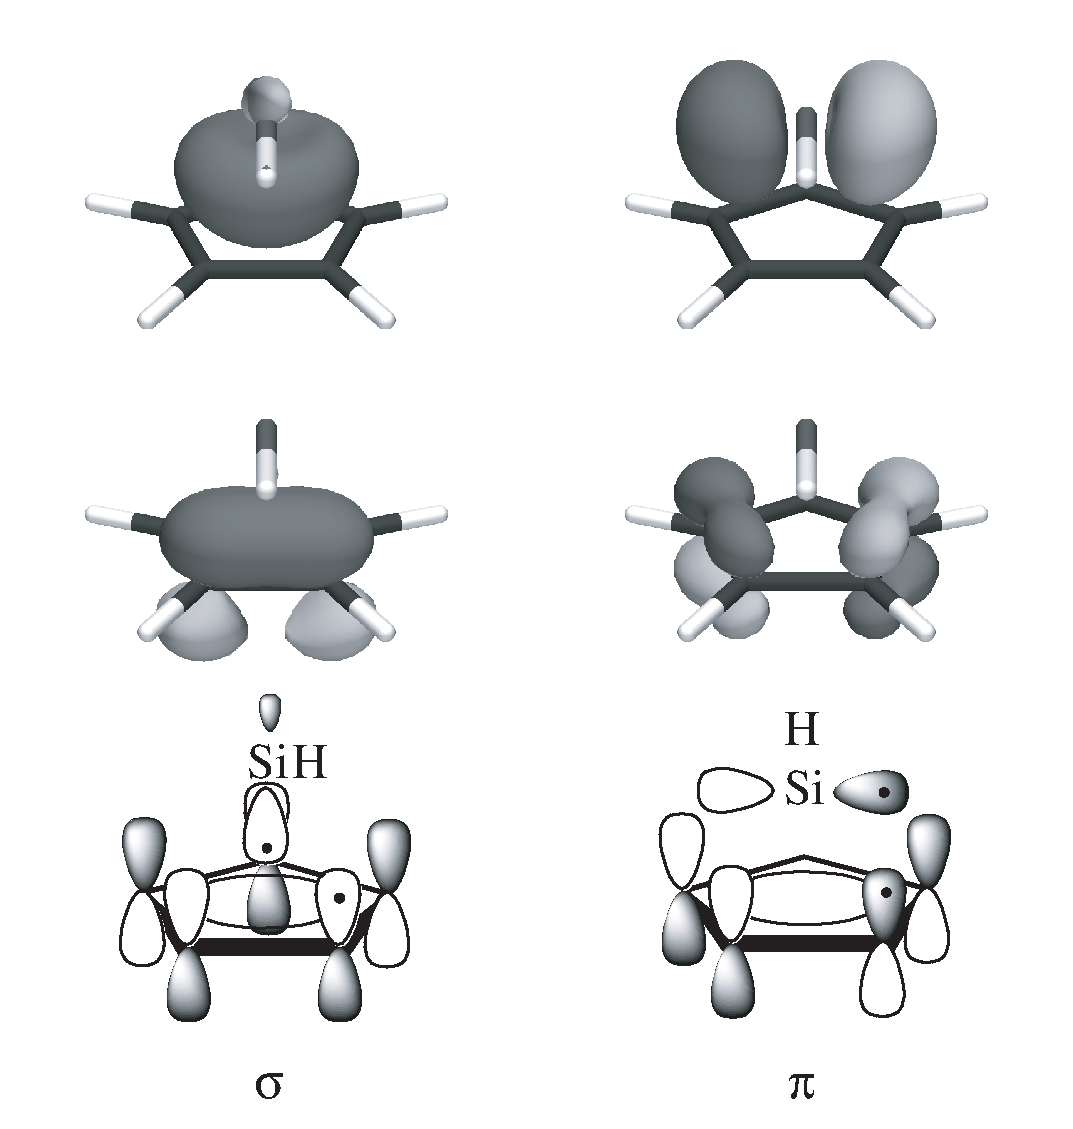
\includegraphics[scale=0.5]{introduction/figures/figure7.eps}
\caption{On the bottom the covalent bond structures are shown, on the left is the $\sigma$ description and on the right is the $\pi$ description. The actual resulting bonding orbitals from the local VBSCF calculation on SiH and Cp are shown on top and in the middle, respectively.}
\label{ch1.fig7}
\end{figure}
The two covalent structures are shown on the bottom in Figure \ref{ch1.fig7}. On the left is the $\sigma$ type bond and on the right a $\pi$ type bond. Both bonds consist of an electron pair of which one electron is located on the siliconhydride part (top) and one on the cyclopentadienyl ring (middle). With the localized orbital model the resulting VB orbitals (top and middle) remain clearly belonging to the separate fragments. 

A drawback of local VBSCF, however, is that it is not very suitable as a quantitative tool: mostly, the total VB energy is higher than for a VBCI calculation with many structures or a delocal VBSCF calculation. And in some cases the use of localized orbitals can even be too restrictive, which might lead to the prediction of a wrong geometry. For example, a calculation on cyclobutadiene with the local VBSCF model \cite{cyclobutt} has shown that the localization of the $p$ orbitals results in a square geometry, rather than the generally accepted rectangular geometry (Figure \ref{ch1.fig.butadiene}) \cite{arnold}. 
\begin{figure}[htdp]
\center
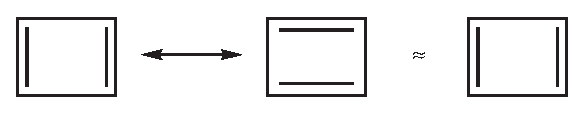
\includegraphics{introduction/figures/butadiene.eps}
\caption{The two Kekul\'e-like resonance structures of cyclobutadiene (left) which is approximately equal to the structure on the right.}
\label{ch1.fig.butadiene}
\end{figure}
From H\"{u}ckel's rule \cite{huckel2,huckel4}, it is expected that planar hydrocarbons ((CH)$_n$) with $4n+2$ $\pi$ electrons are aromatic, while molecules with $4n$ $\pi$ electrons are anti-aromatic. One of the properties of aromatic molecules is their bond length equalization, like in benzene (Figure \ref{ch1.fig.benzene}). For anti-aromatic molecules the double bonds are shorter than the single bonds. The reason for the bond length equilibration for C$_4$H$_4$ in the local VBSCF model is that the $\pi$ bonds are weaker because they have less overlap due to the localization \cite{cyclobutt}. A calculation with the delocal model results in the rectangular geometry \cite{cyclobutt}. Furthermore, in this delocal wave function only one Kekul\'{e}-like structure contributed mainly to the wave function (Figure \ref{ch1.fig.butadiene}, left), resulting in a negligible resonance energy.

In the VB wave functions described so far there is only \textit{one} set of orbitals. In the previous benzene examples (Figure \ref{ch1.fig.structures2}) all structures used the same 6 $2p_z$ orbitals. In the 1990s Hiberty \textit{et al.} introduced the Breathing Orbital Valence Bond method (BOVB). In a BOVB wave function \textit{each structure} has its \textit{own set of orbitals}. For F$_2$, with the structures $\mathrm{[F^\bullet F^\bullet]}$, $\mathrm{[F^{+} F^{-}]}$ and $\mathrm{[F^{-} F^{+}]}$, this means that F$^\bullet$, F$^{-}$ and F$^{+}$ have different orbitals. So, the covalent structure has orbitals optimized for neutral atoms, while the ionic structure has orbitals optimized for charged atoms, which, from an electrostatic point of view, corresponds more to reality than both structures having the same, mostly an average between the two extremes, set of orbitals. The higher versatility of the BOVB method compared to plain VBSCF is reflected in the lower expectation values of the energy, although at cost. Because orbitals in different structures might resemble each other much, \textit{i.e.} have a large overlap, dependencies in the orbital basis can occur, which leads to difficult convergence or no convergence at all.

\subsection{Spin-Coupled Valence Bond (SCVB)}
Cooper, Gerratt and Raimondi have developed the Spin-Coupled Valence Bond (SCVB) method that uses a single reference configuration \cite{scvb1,scvb2,scvb3}. This reference configuration contains doubly and singly occupied orbitals. For the singly occupied orbitals \textit{all} spin-couplings are taken into account. A special form of SCVB is the Complete Active Space Valence Bond (CASVB). As the name of the latter suggests, in CASVB all possible excited structures are generated in the active space. This corresponds to a full CI in the active space. Wave functions of the CAS type are invariant to general transformations and hence the CASVB wave function can be transformed to an (orthogonal) CASSCF wave function. This wave function is optimized (see section \ref{ch1.sec.mcscf}) and transformed back into the CASVB wave function \cite{thor1,thor2,thor3,thor4}.

This method is equivalent with the VBSCF method described in the previous subsection. That is, if in the VBSCF all possible spin-couplings are taken into account. In that case, the expectation value for the total energy ($E_\mathrm{tot}$) will be the same for the same basis set.

\section{Overview of this Thesis}

This thesis consists of three parts: methodology (Chapter \chorbopt), assessment of complex chemical bonding, such as bond making and breaking of dative bonds and bonds with different $\eta$-hapticities (Chapters \chdissociation\ and \chcyclopentadienyl), and aromaticity (Chapters \chhuckel, \chinorganic\ and~\chindacene).

As mentioned earlier, the orbitals in a VB wave function can be optimized with \mbox{VBSCF}. For this optimization a Super CI wave function, containing all possible singly excited structures,  needs to be created. These singly excited structures contain 1-2 times the number of determinants in the ground state wave function. Besides, due to the non-orthogonality, first and second order cofactors, which are signed subdeterminants with orbital overlaps, need to be evaluated.

In Chapter \chorbopt\ the possibilities to bypass these singly excited structures and cofactors are analyzed. In MCSCF, Fock matrices, \textit{i.e.} the matrix representations of the Fock operator on MO basis, have been used for the optimization of doubly occupied orbitals \cite{roos1,roos2}. The analogy between MCSCF and VBSCF, as explained in Section \ref{ch1.sec.vbscf}, justifies a close look at the possible use of a Fock operator in VBSCF. In this chapter the applicability of Fock matrices for the optimization of orbitals in VBSCF is analyzed. Besides, several improvements on the earlier implemented approximated Newton-Raphson technique \cite{koos1} will be presented. The chapter is concluded with some test calculations for which the speed-up factors are compared.

The dissociation behavior of molecules is influenced by the surrounding medium. In Chapter \chdissociation\ this influence is analyzed by comparing the dissociation behavior of four chlorine containing compounds in the gas-phase with in solution. The molecules are chloromethane, \textit{tert}-butylchloride, chlorosilane and trimethylsilylchloride (Figure \ref{ch1.fig.structures1} in which M=C or Si and R=H or CH$_3$).
\begin{figure}[htbp]
\center
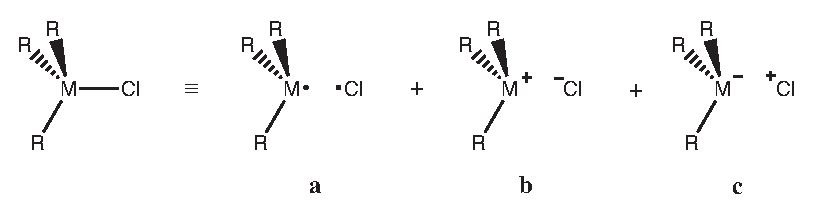
\includegraphics{introduction/figures/structures.eps}
\caption{The total wave function is a combination of three Lewis structures \textbf{a}, \textbf{b} and \textbf{c}, in which M=C or Si and R=H or CH$_3$.}
\label{ch1.fig.structures1}
\end{figure}
The M-Cl bond  is stretched and for several bond lengths the total VB energy and the energy of the separate covalent and ionic structures is calculated. At large distances only the covalent structure (Figure \ref{ch1.fig.structures1}, structure \textbf{a}) contributes to the wave function for the gas-phase. 
 
In computational chemistry, the methods for evaluating solvent effects can be divided into two types: those describing the individual solvent molecules and those that treat the solvent as a continuous medium \cite{jensen}. In continuum models, like the Polarizable Continuum Model (PCM) \cite{pcm1,pcm2}, the solvent is considered to be a uniform polarizable medium with a dielectric constant of $\epsilon$. The solute \textbf{M} is placed in a suitably shaped hole in the medium (figure \ref{ch1.fig.continuum}).
\begin{figure}
\center
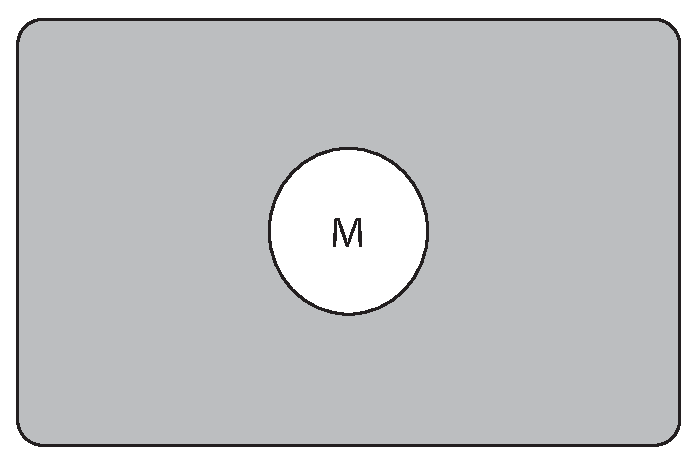
\includegraphics[scale=0.6]{introduction/figures/continuum.eps}
\caption{The solute (\textbf{M}) placed in a suitably shaped hole (white circle), placed in a medium (gray area).}
\label{ch1.fig.continuum}
\end{figure}
In chapter \chdissociation\ the effect of water is mimicked with a value for $\epsilon$ of 78.5. For the holes around the atoms, spheres are chosen. As an estimate for the size, the van der Waals radii of the atoms were taken, scaled by 1.20. The cavity around the molecules therefore becomes shaped liked the molecules themselves. The PCM model changes the energy of the system. Firstly, to create a cavity in the solvent costs energy. On the other hand, the interaction between the solute and the solvent is stabilizing, and hence will lower the energy of the system. 

With PCM switched on \textit{tert}-butylchloride, chlorosilane and trimethylsilylchloride dissociate in ions, \textit{i.e.} at large distances only the ionic structure (Figure \ref{ch1.fig.structures1}, structure \textbf{b}) contributes to the wave function.  Chloromethane is hardly influenced by the solvating medium. At large distances the covalent structure remains the most important for this molecule.  

The cyclopentadienyl anion has 6 $\pi$ electrons and fulfills the 4$n$+2 H\"{u}ckel rule. Although the cyclopentadienyl moiety is frequently used as a ligand in organometallic chemistry (\textit{cf.} ferrocene) details about the actual bond between the metal atom and the ligands are scarce \cite{budzelaar}. In Chapter \chcyclopentadienyl\ the bonding of main-group metal hydrides to a cyclopentadienyl ring is, for which the covalent structures were already shown in Figure \ref{ch1.fig7}, investigated in terms of contributions of VB structures, describing $\sigma$, $\pi$ and ionic bonding (Figure \ref{ch1.fig.mhydride}).
\begin{figure}[ht]
\center
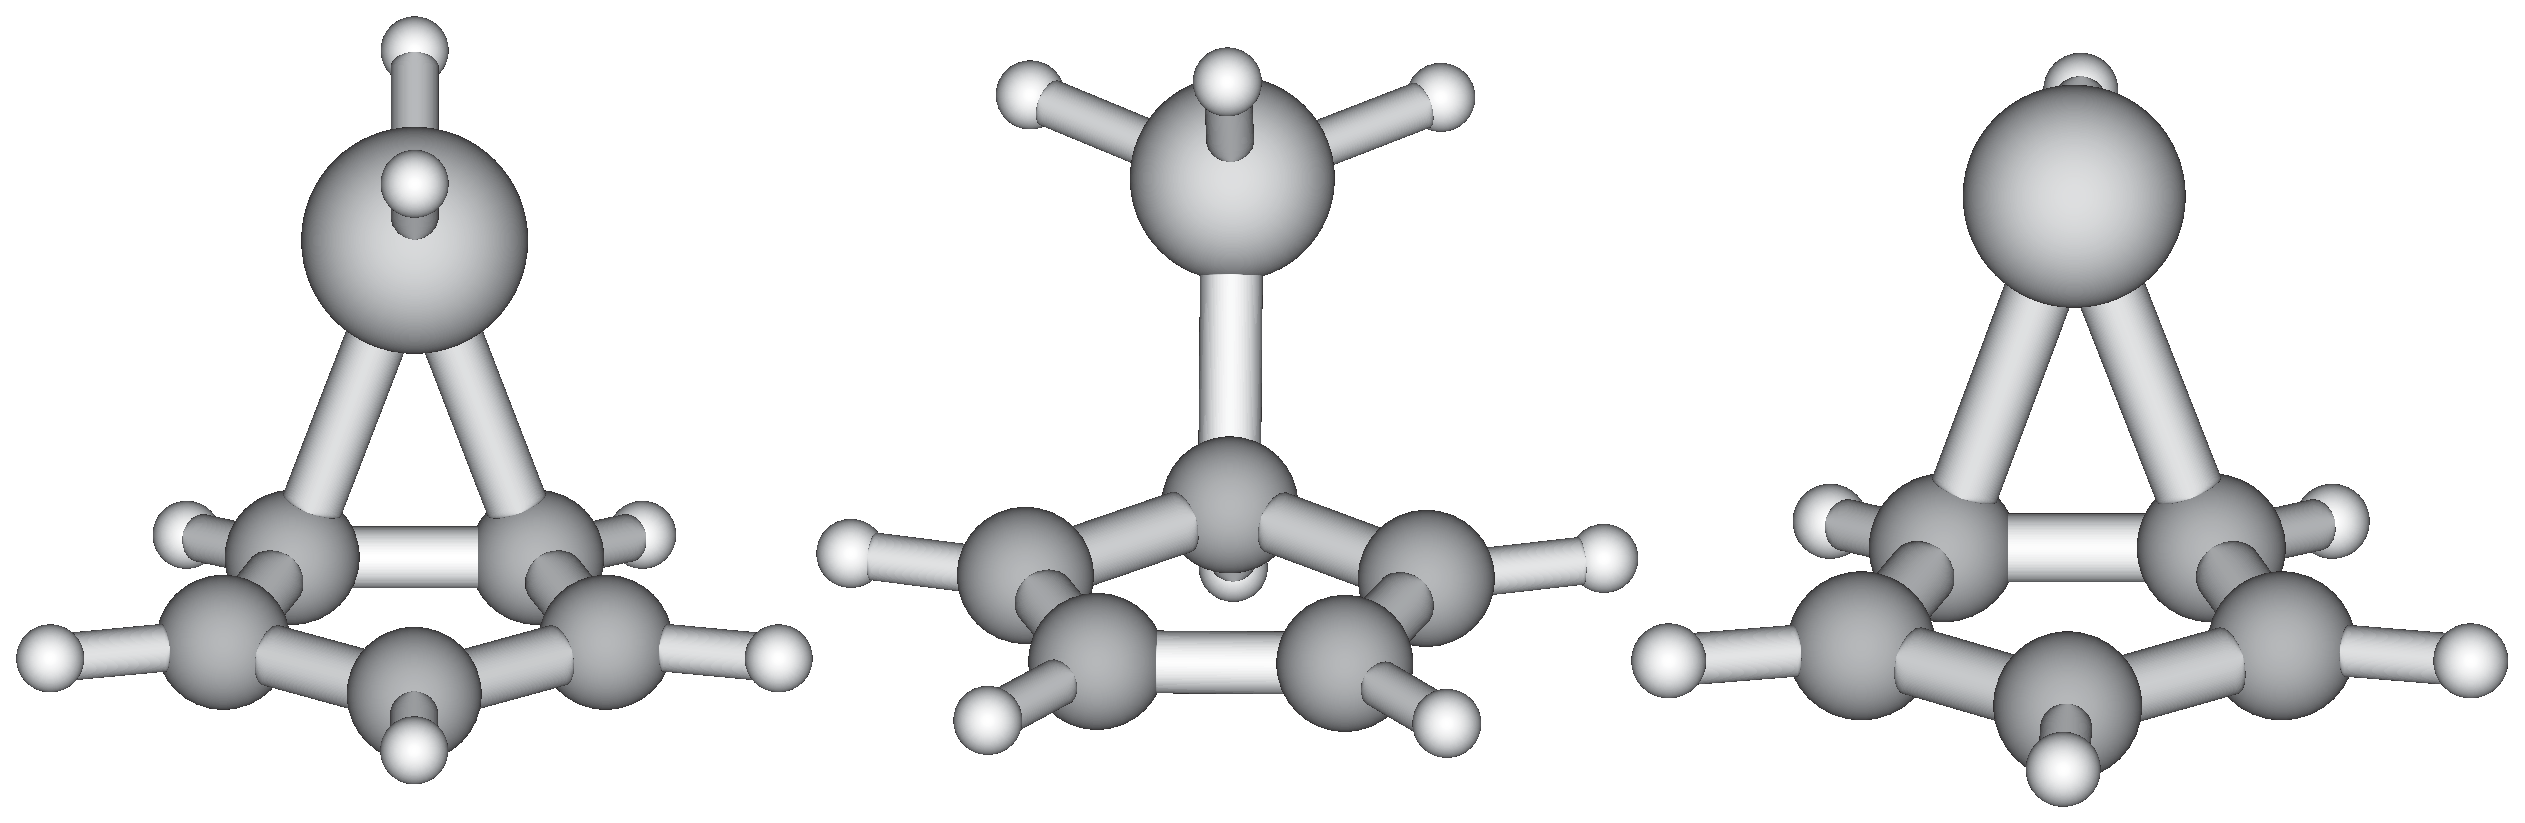
\includegraphics{introduction/figures/mhydride.eps}
\caption{Siliconhydride (left), silicontrihydride (middle) and aluminumdihydride (right) attached to a cyclopentadienyl ring. Please note that the bonds between the ring and the metal hydride are dashed, indicating that these are not actual bonds, nor optimal geometries.}
\label{ch1.fig.mhydride}
\end{figure}

In the last three chapters the aromaticity phenomenon is considered from different perspectives. Since the discovery of benzene in 1825 by Michael Faraday, four criteria for aromaticity have been defined \cite{aromaticity}. These are chemical behavior, structural, energetic and magnetic. In chapters \chhuckel, \chinorganic\ and \chindacene, the latter three criteria have been used in the investigation. 

In aromatic molecules, bond length equalization occurs. This is verified with the several geometry optimizations in the last three chapters of this thesis. Secondly, aromatic molecules have a high resonance energy. Valence Bond theory is well-suited to study this aromatic stability, because a Valence Bond wave function containing both Kekul\'{e} structures can be defined with which the Pauling resonance energy, \textit{i.e.} the energy difference between one Kekul\'e structure and the total energy ($E_\mathrm{tot}$) can be calculated \cite{pauling5} (see figure \ref{ch1.fig.benzene}). The third property used to measure aromaticity is magnetic in nature. Molecules react differently to an external magnetic field. In benzene, for example, the center of the ring is shielded, while the edges of the molecule are deshielded. This phenomenon is measurable with the nucleus-independent chemical shift (NICS) \cite{schleyer}. With this method the absolute magnetic shieldings at the center of the molecular ring are calculated. If a magnetic field is directed perpendicular to the plane of an aromatic system, like benzene, a ring current is induced in the delocalized $\pi$ electrons of the aromatic ring, since these $\pi$ electrons are free to circulate, and hence obey Amp\`{e}re's Law (see Figure \ref{ch1.fig.ringcurrent}).
\begin{figure}[htdp]
\center
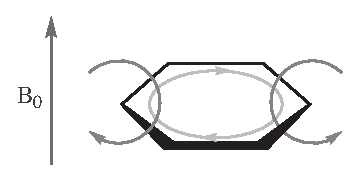
\includegraphics{introduction/figures/ringcurrent.eps}
\caption{A diagram of an aromatic ring current. $\mathrm{B_0}$ is the applied magnetic field, the up-arrow indicating its direction. The arrows in the plane of the atoms shows the direction of the ring current, and the two rings with arrows perpendicular to the C$_6$ ring show the direction of the induced magnetic field.}
\label{ch1.fig.ringcurrent}
\end{figure}
In the last three chapters, the resonance energy calculated with VB will be compared to the ring currents ``measured'' and analyzed whether they corroborate towards the same conclusions: aromatic or anti-aromatic.

The strength of these ring currents can be computed with the ipsocentric CTOCD-DZ (Continuous Transformation
Of Current Density-\textit{Diamagnetic Zero}) method \cite{ctocd1,ctocd2,ctocd3,ctocd4}. With this method an external magnetic field is applied to the molecule and its response to it computed. An advantage of this CTOCD-DZ is that it does not depend on the position of the source of the external magnetic field (gauge independence). For aromatic molecules a diamagnetic ring current will be discernible. The size of the current is expressed in the $j_{max}$ value. For the calculation of the ring currents SYSMO \cite{sysmo} was used.

Benzene fulfills the 4$n$+2 H\"{u}ckel rule for aromatics, while cyclobutadiene and cyclooctatetraene satisfy the 4$n$ rule for anti-aromatics. In Chapter \chhuckel\ the applicability of these rules are tested on the azabora-analogues of these three molecules, which are iso-electronic with their carbon counterparts. Results from a simple H\"{u}ckel model \cite{huckel1,huckel2,huckel3,huckel4}, \textit{ab initio} ring current maps \cite{london,ctocd1,ctocd2,ctocd3,ctocd4}, and the Valence Bond method are compared. A ring current map shows the induced current, caused by a magnetic field, in the electronic system of planar molecules. For aromatic molecules a strong ring current in the $\pi$ system is discernible, whereas for non aromatic molecules only weak currents are visible. Ring current maps are the result of sensitive probing the molecule to assess aromatic character \cite{huckel}.

In Chapter \chinorganic\ the aromaticity of a series of ``inorganic benzenes'', like B$_3$N$_3$H$_6$, B$_3$P$_3$H$_6$ and N$_6$, is investigated. The results of ring current calculations are compared to VB. It is shown that amongst the alleged inorganic benzenes only B$_3$P$_3$H$_6$ (Figure \ref{ch1.fig.b3p3h6}) can be considered as ``aromatic''.
 \begin{figure}[ht]
\center
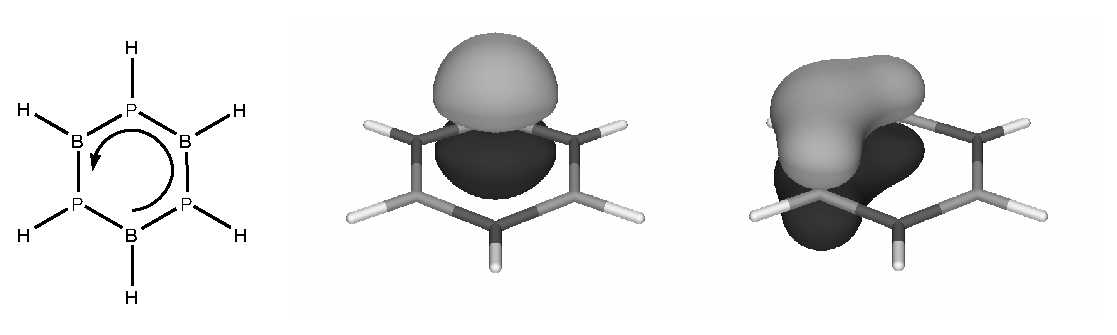
\includegraphics[width=5in]{introduction/figures/b3p3h6.eps}
\caption{Schematic ring current picture of B$_3$P$_3$H$_6$, together with an electron pair (two singly occupied orbitals), as calculated with VB.}
\label{ch1.fig.b3p3h6}
\end{figure}
 Although this molecule is not completely planar in its equilibrium (optimal) geometry, it is also still able to sustain a small induced diatropic ring current \cite{inorganic}.

In Chapter \chindacene\ the aromatic character of compounds fulfilling the 4$n$ H\"{u}ckel rule for anti-aromaticity is examined. In molecules like $s$-indacene the central ring can be regarded as benzene, by drawing the two Kekul\'e-like structures in it. In that case, the two five membered rings will have an unpaired electron, which represents a bi-radical (Figure \ref{ch1.fig.indacene}). 
\begin{figure}[htdp]
\center
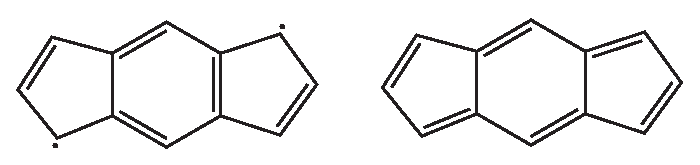
\includegraphics{introduction/figures/indacene.eps}
\caption{A structure with a Kekul\'e ring in the middle and two unpaired electrons (left) and a structure without bi-radical character of \textit{s}-indacene.}
\label{ch1.fig.indacene}
\end{figure}
In VB structures without bi-radical character, it is impossible to have Kekul\'e-like structures in the central ring, which has only two instead of three double bonds (Figure \ref{ch1.fig.indacene} (right)). By increasing the number of six membered rings, the aromatic character is expected to increase, resulting in more bi-radical character in the five membered rings. These effects are studied both with the Valence Bond method and \textit{ab initio} ring current mapping \cite{indacene}.  

\bibliography{introduction}
\bibliographystyle{../main/achemso} 
